Dans cette section, nous présentons les principales interfaces développées durant ce premier sprint, en commençant par la page d’accueil, puis celles liées au module d’authentification, et enfin les interfaces de contact et d'administration des utilisateurs.
\begin{itemize}[label=$\bullet$]
    \item  \textbf{Interface de la page d’accueil}: Les figures\footnote{Voir annexe E : Figures \ref{fig:accueil} et \ref{fig:accueil2}} \ref{fig:accueil} et \ref{fig:accueil2} illustrent l’interface de la page d’accueil de l’application. Celle-ci offre un aperçu général du système, avec un design moderne et une navigation intuitive, permettant aux utilisateurs de découvrir rapidement les principales fonctionnalités de la plateforme.
    \item \textbf{Interface d’inscription}:
        La figure~\ref{fig:register} illustre l’interface d’inscription. Elle permet à un nouvel utilisateur de créer un compte en renseignant ses informations personnelles. Des contrôles de saisie assurent la validation des données entrées.  
        \begin{figure}[H]
            \centering
            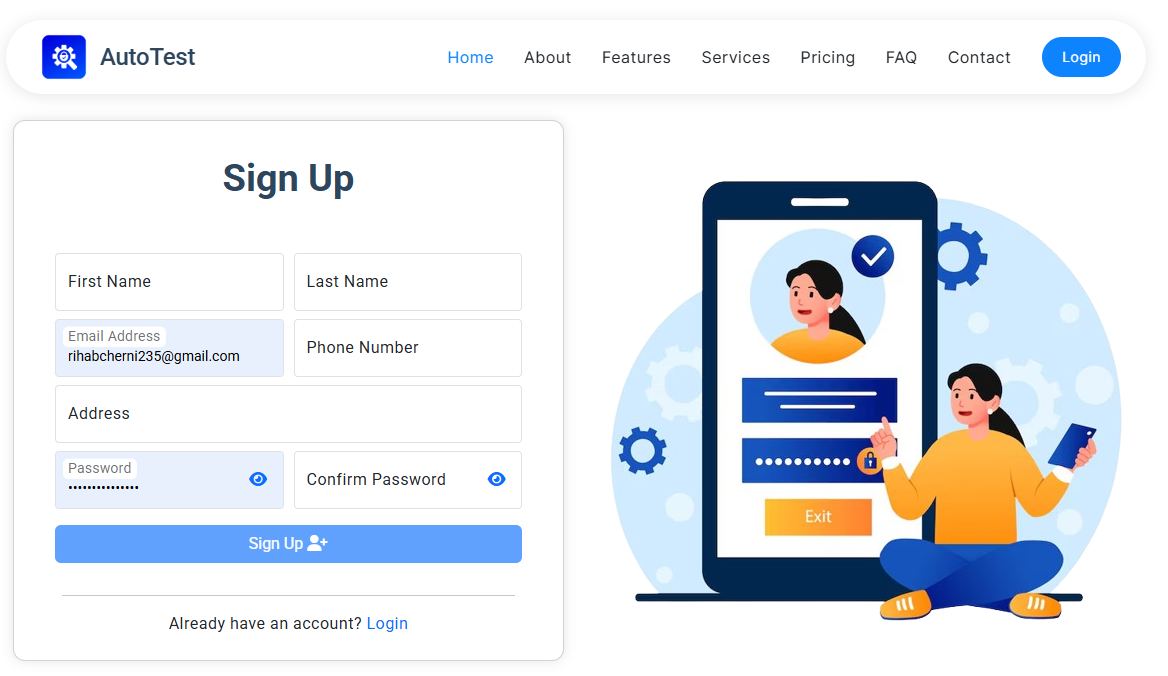
\includegraphics[width=\linewidth]{chapitres/ch3Sp1/section/sprint1/img/interface/register.png}
            \caption{\centering Interface d'inscription}
            \label{fig:register}
        \end{figure}
        \vspace{-0.3cm}
    \item \textbf{Interface de connexion}:
        La figure~\ref{fig:login}\footnote{Voir annexe E: Figures \ref{fig:login}} présente l’interface de connexion. Elle permet à l’utilisateur de s’authentifier via son e-mail et son mot de passe. Des vérifications sont mises en place pour gérer les erreurs (identifiants invalides, champs manquants...).
    \item \textbf{Vérification par e-mail (OTP)}:
        Après l’inscription, l’utilisateur reçoit un e-mail contenant un code de vérification. Les figures \ref{fig:email-verif}\footnote{Voir annexe E: Figures \ref{fig:email-verif}} et \ref{fig:email-verification}\footnote{Voir annexe E: Figures \ref{fig:email-verification}} présentent l’interface de réception et de saisie du code.
    \item \textbf{Mot de passe oublié et réinitialisation}:
        Le système inclut une fonctionnalité de récupération de mot de passe. Les interfaces correspondantes sont illustrées dans les figures~\ref{fig:forgot-password}\footnote{Voir annexe E: Figures \ref{fig:forgot-password}},~\ref{fig:reset-password-email}\footnote{Voir annexe E: Figures \ref{fig:reset-password-email}} et~\ref{fig:reset-password}\footnote{Voir annexe E: Figures \ref{fig:reset-password}}.
        \item \textbf{Profil utilisateur} : La figure~\ref{fig:profile} présente l’interface du profil utilisateur. Chaque utilisateur peut consulter et modifier ses informations personnelles (nom, image de profil, etc.), ainsi que visualiser les permissions qui lui sont attribuées. \\ Un bouton dédié permet également à l’utilisateur de soumettre une demande d’accès à des permissions supplémentaires via une boîte de dialogue affichant la liste des permissions disponibles, que l’utilisateur peut sélectionner avant de valider sa demande.
         \begin{figure}[H]
                \centering
                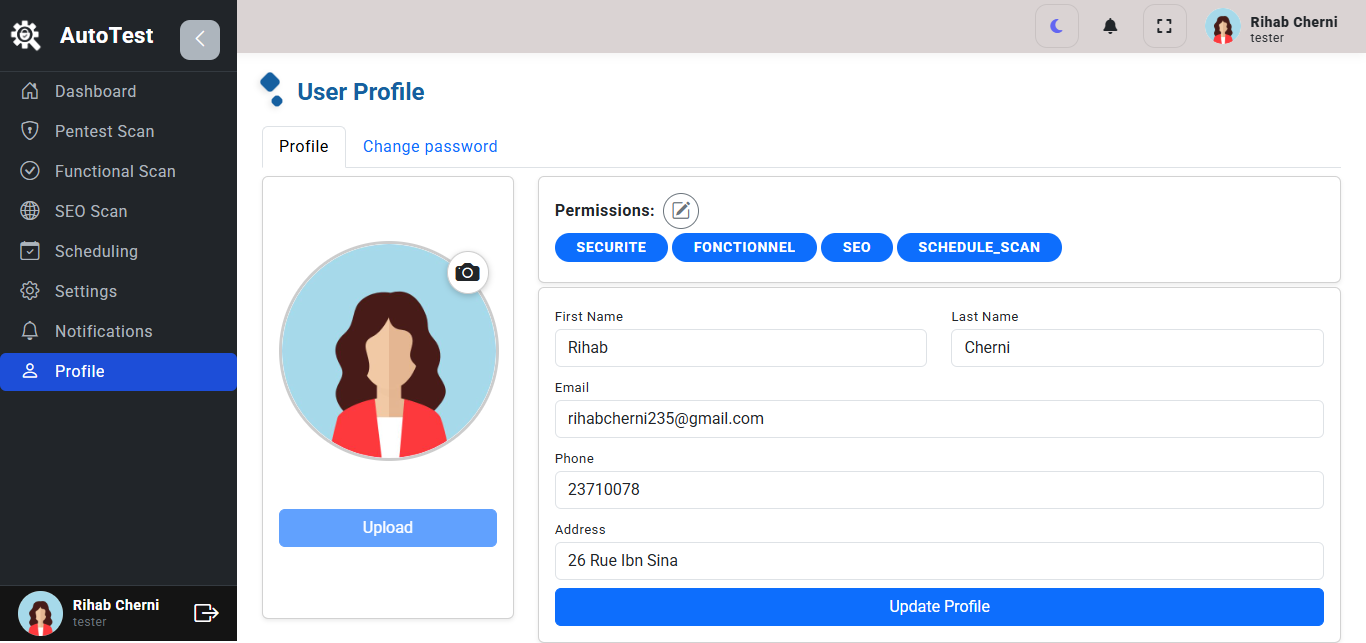
\includegraphics[width=\linewidth]{chapitres/ch3Sp1/section/sprint1/img/interface/profile.png}
                \caption{\centering Interface du profil utilisateur}
                \label{fig:profile}
            \end{figure}
        \vspace{-0.3cm}
    \item \textbf{Gestion des utilisateurs et permissions}:
        La figure~\ref{fig:gestionUser} présente l’interface dédiée à la gestion des utilisateurs pour l’administrateur. Elle permet de visualiser, rechercher, modifier ou supprimer les comptes utilisateurs, de gérer les permissions attribuées à chacun, et d’exporter la liste aux différents formats disponibles.
        \begin{figure}[H]
            \centering
            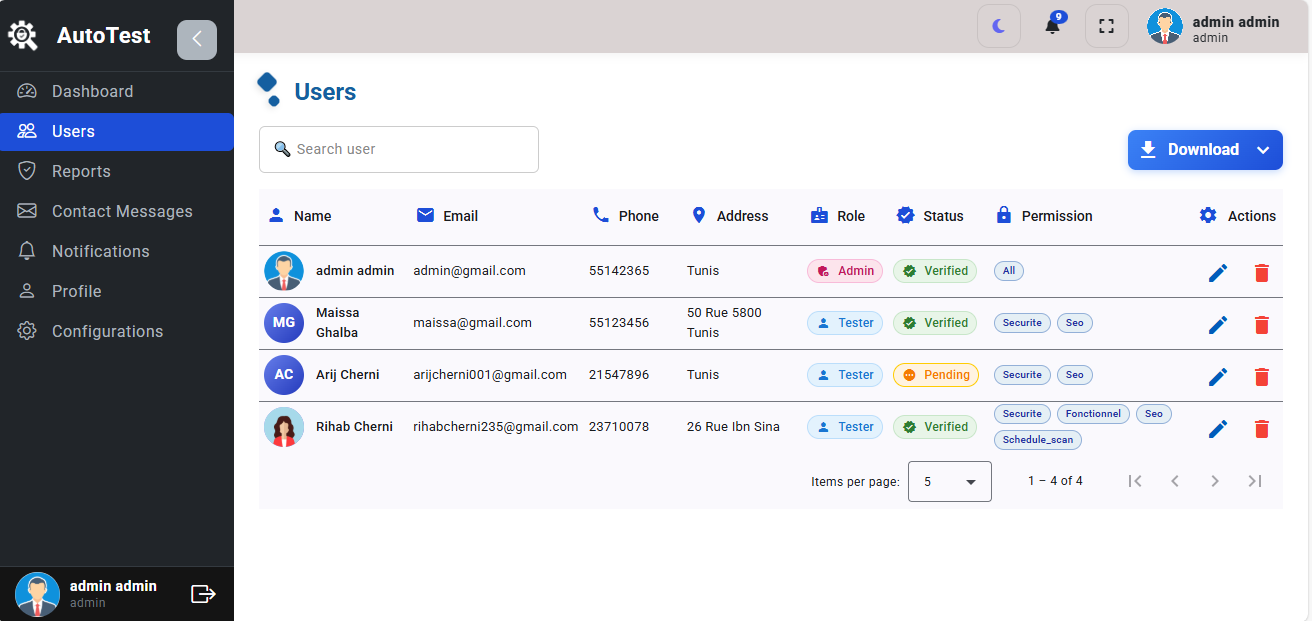
\includegraphics[width=\linewidth]{chapitres/ch3Sp1/section/sprint1/img/interface/user-liste.PNG}
            \caption{\centering Interface de gestion des utilisateurs et permissions (admin)}
            \label{fig:gestionUser}
        \end{figure}
        \vspace{-0.3cm}
       \item \textbf{Interfaces liées à la gestion des permissions et guards} :
Cette partie décrit les interfaces conditionnées par le système de gestion des permissions et les guards de sécurité implémentés dans l’application.
\begin{itemize}[label=$\diamond$, left=0.01cm]
    \item \textbf{Menu latéral dynamique selon les permissions} : La figure~\ref{fig:sidebar}\footnote{Voir annexe E : Figure~\ref{fig:sidebar}} illustre l’adaptation dynamique du menu latéral en fonction des droits d’accès de l’utilisateur. Trois cas sont représentés : (a) un utilisateur sans permissions, où seuls les éléments de base (profil, paramètres) sont visibles, (b) un utilisateur disposant de permissions spécifiques accédant uniquement aux modules autorisés, et (c) un utilisateur avec l’ensemble des droits, ayant un accès complet aux modules (SEO, sécurité, tests fonctionnels, génération de rapports, ...).
        \item \textbf{Interfaces de gestion des permissions}: La figure~\ref{fig:permission-interfaces}\footnote{Voir annexe E: Figures \ref{fig:permission-interfaces}} présente les interfaces illustrant les mécanismes de gestion et de demande de permissions.    
        \begin{itemize}[label=$*$, left=0.01cm]
            \item (a) Boîte de dialogue des permissions pour l’administrateur, avec toutes les permissions cochées et désactivées grâce à la permission spéciale \texttt{tous}, accordant un accès complet.
            \item (b) Boîte de dialogue d’édition des permissions, accessible uniquement à l’administrateur, permettant d’ajouter ou de révoquer dynamiquement les droits d’un utilisateur de rôle \texttt{testeur}.
            \item (c) Interface de demande de permissions, permettant au testeur de visualiser les accès manquants et de soumettre une requête à l’administrateur. Une notification est automatiquement envoyée. Ce composant a été conçu avec une logique évolutive en vue de la commercialisation de l’application : certaines permissions pourront, à l’avenir, être conditionnées par un abonnement payant. Une option de paiement ou un lien vers la facturation pourra alors s’activer dynamiquement lors de la sélection.
    \end{itemize}
\end{itemize}
\item \textbf{Soumettre un message de contact}:
        L’interface illustrée dans la figure~\ref{fig:contact}\footnote{Voir annexe E: Figures \ref{fig:contact}} permet à tout utilisateur (même non connecté) de soumettre un message à l’administrateur.
    \item \textbf{Interface de liste des messages (côté administrateur)}:
        La figure~\ref{fig:admin-contact-list}\footnote{Voir annexe E: Figures \ref{fig:admin-contact-list}} montre l’interface accessible uniquement à l’administrateur, lui permettant de consulter la liste des messages reçus via le formulaire de contact.
\end{itemize}